% Options for packages loaded elsewhere
\PassOptionsToPackage{unicode}{hyperref}
\PassOptionsToPackage{hyphens}{url}
%
\documentclass[
]{article}
\usepackage{amsmath,amssymb}
\usepackage{lmodern}
\usepackage{ifxetex,ifluatex}
\ifnum 0\ifxetex 1\fi\ifluatex 1\fi=0 % if pdftex
  \usepackage[T1]{fontenc}
  \usepackage[utf8]{inputenc}
  \usepackage{textcomp} % provide euro and other symbols
\else % if luatex or xetex
  \usepackage{unicode-math}
  \defaultfontfeatures{Scale=MatchLowercase}
  \defaultfontfeatures[\rmfamily]{Ligatures=TeX,Scale=1}
\fi
% Use upquote if available, for straight quotes in verbatim environments
\IfFileExists{upquote.sty}{\usepackage{upquote}}{}
\IfFileExists{microtype.sty}{% use microtype if available
  \usepackage[]{microtype}
  \UseMicrotypeSet[protrusion]{basicmath} % disable protrusion for tt fonts
}{}
\makeatletter
\@ifundefined{KOMAClassName}{% if non-KOMA class
  \IfFileExists{parskip.sty}{%
    \usepackage{parskip}
  }{% else
    \setlength{\parindent}{0pt}
    \setlength{\parskip}{6pt plus 2pt minus 1pt}}
}{% if KOMA class
  \KOMAoptions{parskip=half}}
\makeatother
\usepackage{xcolor}
\IfFileExists{xurl.sty}{\usepackage{xurl}}{} % add URL line breaks if available
\IfFileExists{bookmark.sty}{\usepackage{bookmark}}{\usepackage{hyperref}}
\hypersetup{
  hidelinks,
  pdfcreator={LaTeX via pandoc}}
\urlstyle{same} % disable monospaced font for URLs
\usepackage[margin=1in]{geometry}
\usepackage{color}
\usepackage{fancyvrb}
\newcommand{\VerbBar}{|}
\newcommand{\VERB}{\Verb[commandchars=\\\{\}]}
\DefineVerbatimEnvironment{Highlighting}{Verbatim}{commandchars=\\\{\}}
% Add ',fontsize=\small' for more characters per line
\usepackage{framed}
\definecolor{shadecolor}{RGB}{248,248,248}
\newenvironment{Shaded}{\begin{snugshade}}{\end{snugshade}}
\newcommand{\AlertTok}[1]{\textcolor[rgb]{0.94,0.16,0.16}{#1}}
\newcommand{\AnnotationTok}[1]{\textcolor[rgb]{0.56,0.35,0.01}{\textbf{\textit{#1}}}}
\newcommand{\AttributeTok}[1]{\textcolor[rgb]{0.77,0.63,0.00}{#1}}
\newcommand{\BaseNTok}[1]{\textcolor[rgb]{0.00,0.00,0.81}{#1}}
\newcommand{\BuiltInTok}[1]{#1}
\newcommand{\CharTok}[1]{\textcolor[rgb]{0.31,0.60,0.02}{#1}}
\newcommand{\CommentTok}[1]{\textcolor[rgb]{0.56,0.35,0.01}{\textit{#1}}}
\newcommand{\CommentVarTok}[1]{\textcolor[rgb]{0.56,0.35,0.01}{\textbf{\textit{#1}}}}
\newcommand{\ConstantTok}[1]{\textcolor[rgb]{0.00,0.00,0.00}{#1}}
\newcommand{\ControlFlowTok}[1]{\textcolor[rgb]{0.13,0.29,0.53}{\textbf{#1}}}
\newcommand{\DataTypeTok}[1]{\textcolor[rgb]{0.13,0.29,0.53}{#1}}
\newcommand{\DecValTok}[1]{\textcolor[rgb]{0.00,0.00,0.81}{#1}}
\newcommand{\DocumentationTok}[1]{\textcolor[rgb]{0.56,0.35,0.01}{\textbf{\textit{#1}}}}
\newcommand{\ErrorTok}[1]{\textcolor[rgb]{0.64,0.00,0.00}{\textbf{#1}}}
\newcommand{\ExtensionTok}[1]{#1}
\newcommand{\FloatTok}[1]{\textcolor[rgb]{0.00,0.00,0.81}{#1}}
\newcommand{\FunctionTok}[1]{\textcolor[rgb]{0.00,0.00,0.00}{#1}}
\newcommand{\ImportTok}[1]{#1}
\newcommand{\InformationTok}[1]{\textcolor[rgb]{0.56,0.35,0.01}{\textbf{\textit{#1}}}}
\newcommand{\KeywordTok}[1]{\textcolor[rgb]{0.13,0.29,0.53}{\textbf{#1}}}
\newcommand{\NormalTok}[1]{#1}
\newcommand{\OperatorTok}[1]{\textcolor[rgb]{0.81,0.36,0.00}{\textbf{#1}}}
\newcommand{\OtherTok}[1]{\textcolor[rgb]{0.56,0.35,0.01}{#1}}
\newcommand{\PreprocessorTok}[1]{\textcolor[rgb]{0.56,0.35,0.01}{\textit{#1}}}
\newcommand{\RegionMarkerTok}[1]{#1}
\newcommand{\SpecialCharTok}[1]{\textcolor[rgb]{0.00,0.00,0.00}{#1}}
\newcommand{\SpecialStringTok}[1]{\textcolor[rgb]{0.31,0.60,0.02}{#1}}
\newcommand{\StringTok}[1]{\textcolor[rgb]{0.31,0.60,0.02}{#1}}
\newcommand{\VariableTok}[1]{\textcolor[rgb]{0.00,0.00,0.00}{#1}}
\newcommand{\VerbatimStringTok}[1]{\textcolor[rgb]{0.31,0.60,0.02}{#1}}
\newcommand{\WarningTok}[1]{\textcolor[rgb]{0.56,0.35,0.01}{\textbf{\textit{#1}}}}
\usepackage{graphicx}
\makeatletter
\def\maxwidth{\ifdim\Gin@nat@width>\linewidth\linewidth\else\Gin@nat@width\fi}
\def\maxheight{\ifdim\Gin@nat@height>\textheight\textheight\else\Gin@nat@height\fi}
\makeatother
% Scale images if necessary, so that they will not overflow the page
% margins by default, and it is still possible to overwrite the defaults
% using explicit options in \includegraphics[width, height, ...]{}
\setkeys{Gin}{width=\maxwidth,height=\maxheight,keepaspectratio}
% Set default figure placement to htbp
\makeatletter
\def\fps@figure{htbp}
\makeatother
\setlength{\emergencystretch}{3em} % prevent overfull lines
\providecommand{\tightlist}{%
  \setlength{\itemsep}{0pt}\setlength{\parskip}{0pt}}
\setcounter{secnumdepth}{-\maxdimen} % remove section numbering
\usepackage{enumitem}
\usepackage{caption}
\usepackage{amsmath}
\captionsetup{labelformat=empty}
\usepackage[utf8]{inputenc}
\usepackage{geometry}
\usepackage{amsmath}
\usepackage{amssymb}
\usepackage{tabularx}
\ifluatex
  \usepackage{selnolig}  % disable illegal ligatures
\fi

\author{}
\date{\vspace{-2.5em}}

\begin{document}

\begin{center}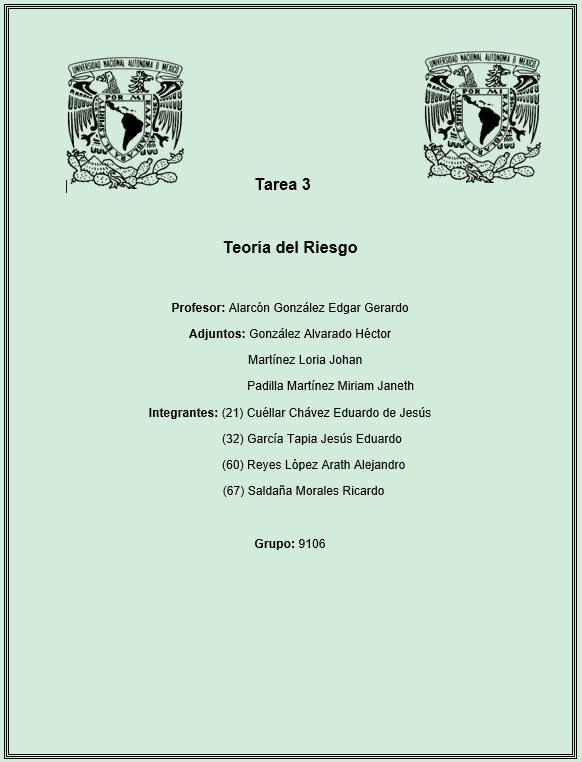
\includegraphics[width=2.4\linewidth]{CARATULA} \end{center}
\newpage

Realiza los siguientes ejercicios cuidando el formato y las reglas
establecidas en la presentación del curso. Sube las soluciones a
\emph{Classroom} dentro del apartado correspondiente a esta tarea en
archivos \textbf{NO COMRPIMIDOS}.

Realiza los siguientes ejercicios entregando el desarrollo algebraico
por escrito (a mano) y las conclusiones del mismo en un archivo de
\textbf{R Markdown con su respectivo compilado PDF} impreso y por correo
electrónico (todos los ejercicios valen lo mismo).

\hypertarget{ejercicio-1}{%
\section{Ejercicio 1}\label{ejercicio-1}}

Sea S un modelo colectivo (compuesto) con frecuencia \(N\sim Bin(n,p)\)
y severidad \(Y\sim Ber(\theta)\). Calcula:

\begin{enumerate}[label=(\alph*)]
\item  $\mathbb{E}[S]$
\item  $Var(S)$
\item  $M_S(t)$
\item Di qué distribución tiene $S$ especificando sus parámetros.
\end{enumerate}

\hypertarget{soluciuxf3n}{%
\subsubsection{Solución}\label{soluciuxf3n}}

\hypertarget{inciso-a}{%
\subsection{Inciso a)}\label{inciso-a}}

Como \begin{align*}
\mathbb{E}[S] &= \mathbb{E}[N] \mathbb{E}[Y]\\
              &= np(\theta)\\
              &= np\theta\\
\therefore \mathbb{E}[S] &= np\theta_\blacksquare
\end{align*}

\hypertarget{inciso-b}{%
\subsection{Inciso b)}\label{inciso-b}}

Como \begin{align*}
Var(S) &= Var(N) \mathbb{E}^{2}(Y) + Var(Y) \mathbb{E}(N)\\
       &= [np(1-p)]\theta^{2} + [\theta(1 - \theta)] np\\
\therefore Var(S) &= [np(1-p)]\theta^{2} + [\theta(1 - \theta)] np_\blacksquare
\end{align*}

\hypertarget{inciso-c}{%
\subsection{Inciso c)}\label{inciso-c}}

Como \begin{align*}
M_{S}(t) &= M_{N} (ln(M_{Y}(t)))\\
\text{Y como} \quad M_{N}(t) &= (1-p + pe^{t})^{n}\\
              M_{Y}(t) &= (1 - \theta + \theta e^{t})\\
              &\implies ln(M_{Y}(t)) = ln(1 - \theta + \theta e^{t})\\
              &\implies M_{S}(t) = (1 - p + p e^{ln(1 - \theta + \theta e^{t})})^{n}\\
              &= (1 - p + p (1 - \theta + \theta e^{t}))^{n}\\
              &= (1 \textcolor{red}{- p + p} - \theta p + \theta p e^{t})^{n}\\
              &= (1 - \theta p + \theta p e^{t})^{n}\\
\therefore M_{S}(t) &= (1 - \theta p + \theta p e^{t})^{n}_\blacksquare
\end{align*}

\hypertarget{inciso-d}{%
\subsection{Inciso d)}\label{inciso-d}}

Notemos que
\(S \sim \text{Binomial compuesta} (n,p,b = Bernoulli(\theta))\)

Además, de manera más especifica;
\(S \sim \text{Binomial}(n, \theta p) \quad \text{por su fmg.}_\blacksquare\)

\hypertarget{ejercicio-2}{%
\section{Ejercicio 2}\label{ejercicio-2}}

Sea S un modelo colectivo (compuesto) con frecuencia
\(N\sim BinNeg(r,p)\) y severidad \(Y\sim Ber(\theta)\). Calcula:

\begin{enumerate}[label=(\alph*)]
\item  $\mathbb{E}[S]$
\item  $Var(S)$
\item  $M_S(t)$
\item Di qué distribución tiene $S$ especificando sus parámetros.
\end{enumerate}

\hypertarget{soluciuxf3n-1}{%
\subsubsection{Solución}\label{soluciuxf3n-1}}

\hypertarget{inciso-a-1}{%
\subsection{Inciso a)}\label{inciso-a-1}}

Como \begin{align*}
\mathbb{E}[S] &= \mathbb{E}[N] \mathbb{E}[Y]\\
              &= \frac{r (1 - p)}{p}(\theta)\\
              &= r\theta \left(\frac{1}{p} - 1\right)\\
\therefore \mathbb{E}[S] &= r\theta \left(\frac{1}{p} - 1\right)_\blacksquare
\end{align*}

\hypertarget{inciso-b-1}{%
\subsection{Inciso b)}\label{inciso-b-1}}

Como \begin{align*}
Var(S) &= Var(N) \mathbb{E}^{2}(Y) + Var(Y) \mathbb{E}(N)\\
       &= \frac{r(1 - p)}{p^{2}}\theta^{2} + [\theta(1 - \theta)] \frac{r (1 - p)}{p}\\
\therefore Var(S) &= \frac{r(1 - p)}{p^{2}}\theta^{2} + [\theta(1 - \theta)] \frac{r (1 - p)}{p}_\blacksquare
\end{align*}

\hypertarget{inciso-c-1}{%
\subsection{Inciso c)}\label{inciso-c-1}}

Como \begin{align*}
M_{S}(t) &= M_{N} (ln(M_{Y}(t)))\\
\text{Y como} \quad M_{N}(t) &= \left[\frac{p}{1 - (1 - p)e^{t}}\right]^{r}\\
              M_{Y}(t) &= (1 - \theta + \theta e^{t})\\
              &\implies ln(M_{Y}(t)) = ln(1 - \theta + \theta e^{t})\\
              &\implies M_{S}(t) = \left[\frac{p}{1 - (1 - p) e^{ln(1 - \theta + \theta e^{t})}}\right]^{r}\\
\textcolor{blue}{(1)} &= \left[\frac{p}{1 - (1 - p) \left[1 - \theta + \theta e^{t}\right]}\right]^{r}\\
\therefore M_{S}(t) &= \left[\frac{p}{1 - (1 - p) \left[1 - \theta + \theta e^{t}\right]}\right]^{r}_\blacksquare
\end{align*}

\hypertarget{inciso-d-1}{%
\subsection{Inciso d)}\label{inciso-d-1}}

Notemos que
\(S \sim \text{Binomial negativa compuesta} (k,p,b = Bernoulli(\theta))_\blacksquare\)

\hypertarget{ejercicio-3}{%
\section{Ejercicio 3}\label{ejercicio-3}}

Considera los siguientes 3 riesgos de una compañía:

\[S_j\sim\text{PoiComp}\left(\lambda_j=j^2,F_{Y_j}\right)\]

Donde las severidades están dadas por:

\begin{itemize}
\tightlist
\item
  \(F_{Y_1}(y)=1-e^{-0.5y} \mathbb{I}^{(y)}_{\{y>0\}}\)
\item
  \(Y_2\) pertenece a la clase (a,b,0) con: \(a=0.1\) , \(b=2(0.1)\) y
  \(p_0=(0.9)^{3}\)
\item
  \(Y_3\) es la v.a. del monto de pérdida de una compañía de seguros con
  un \textbf{contrato de monto máximo de beneficio} \(u=50\) donde el
  monto de pérdida del siniestro es
  \(X\sim Exp\left(\lambda=\frac{1}{100}\right)\) (\(E[X]=100\)).
\end{itemize}

Define el riesgo \(S\) de la compañía como:

\[S=\sum_{j=1}^{3} S_j\]

\textbf{Fija la semilla en 6}, simula \(n=1,000,000\) observaciones de
\(S\) y calcula de manera muestral:

\begin{enumerate}[label=(\alph*)]
\item  El coeficiente de variación de $S$.
\item  Un valor $z$ tal que $F_S(500)\approx \Phi(z)$.
\end{enumerate}

\begin{Shaded}
\begin{Highlighting}[]
\FunctionTok{library}\NormalTok{(actuar)}
\NormalTok{n }\OtherTok{\textless{}{-}} \DecValTok{1000000}
\FunctionTok{set.seed}\NormalTok{(}\DecValTok{6}\NormalTok{)}

\CommentTok{\#Parámetro de la Poisson}
\NormalTok{lambda1 }\OtherTok{\textless{}{-}} \DecValTok{1}\SpecialCharTok{\^{}}\DecValTok{2}
\NormalTok{lambda2 }\OtherTok{\textless{}{-}} \DecValTok{2}\SpecialCharTok{\^{}}\DecValTok{2}
\NormalTok{lambda3 }\OtherTok{\textless{}{-}} \DecValTok{3}\SpecialCharTok{\^{}}\DecValTok{2}
\NormalTok{lambda }\OtherTok{\textless{}{-}}\NormalTok{ lambda1 }\SpecialCharTok{+}\NormalTok{ lambda2 }\SpecialCharTok{+}\NormalTok{ lambda3}

\CommentTok{\#Binomial negativa}
\NormalTok{r}\OtherTok{=}\DecValTok{3}
\NormalTok{p}\OtherTok{=}\FloatTok{0.9}
\NormalTok{S1 }\OtherTok{\textless{}{-}} \FunctionTok{rcompound}\NormalTok{(}\AttributeTok{n =}\NormalTok{ n, }\CommentTok{\#Genera n}
                \AttributeTok{model.freq =} \FunctionTok{rpois}\NormalTok{(}\AttributeTok{lambda =}\NormalTok{ lambda1), }\CommentTok{\#N\textasciitilde{}Poi(lambda1)}
                \AttributeTok{model.sev =} \FunctionTok{rnbinom}\NormalTok{(}\AttributeTok{size =}\NormalTok{ r,}\AttributeTok{p=}\NormalTok{p)) }\CommentTok{\#Y\textasciitilde{}NegBinom(r=3,p=0.9) }

\CommentTok{\#Exponencial}
\NormalTok{rate\_1 }\OtherTok{\textless{}{-}} \DecValTok{1}\SpecialCharTok{/}\DecValTok{2}
\NormalTok{S2 }\OtherTok{\textless{}{-}} \FunctionTok{rcompound}\NormalTok{(}\AttributeTok{n =}\NormalTok{ n, }\CommentTok{\#Genera n}
               \AttributeTok{model.freq =} \FunctionTok{rpois}\NormalTok{(}\AttributeTok{lambda =}\NormalTok{ lambda2), }\CommentTok{\#N\textasciitilde{}Poi(lambda2)}
               \AttributeTok{model.sev =} \FunctionTok{rexp}\NormalTok{(}\AttributeTok{rate =}\NormalTok{ rate\_1)) }\CommentTok{\#Y\textasciitilde{}Exp(rate) }

\CommentTok{\#Exponencial topada}
\NormalTok{rate\_2}\OtherTok{\textless{}{-}} \DecValTok{1}\SpecialCharTok{/}\DecValTok{100}
\NormalTok{u}\OtherTok{=}\DecValTok{50}
\NormalTok{aux}\OtherTok{\textless{}{-}}\ControlFlowTok{function}\NormalTok{(n,rate,u)\{ }\CommentTok{\#Exponencial topada a 50}
  \FunctionTok{return}\NormalTok{(}\FunctionTok{pmin}\NormalTok{(}\FunctionTok{rexp}\NormalTok{(}\AttributeTok{n=}\NormalTok{n,}\AttributeTok{rate=}\NormalTok{rate),u))}
\NormalTok{\}}
\NormalTok{S3 }\OtherTok{\textless{}{-}} \FunctionTok{rcompound}\NormalTok{(}\AttributeTok{n =}\NormalTok{ n, }\CommentTok{\#Genera n}
                \AttributeTok{model.freq =} \FunctionTok{rpois}\NormalTok{(}\AttributeTok{lambda =}\NormalTok{ lambda3), }\CommentTok{\#N\textasciitilde{}Poi(lambda3)}
                \AttributeTok{model.sev =} \FunctionTok{aux}\NormalTok{(}\AttributeTok{rate=}\NormalTok{rate\_2,u)) }\CommentTok{\#Y:=min(Exp(1/100),50)}
\NormalTok{S }\OtherTok{\textless{}{-}}\NormalTok{ S1 }\SpecialCharTok{+}\NormalTok{ S2 }\SpecialCharTok{+}\NormalTok{ S3}

\CommentTok{\#Teórica}
\NormalTok{mu\_nbinom}\OtherTok{=}\NormalTok{r}\SpecialCharTok{*}\NormalTok{(}\DecValTok{1}\SpecialCharTok{/}\NormalTok{p}\DecValTok{{-}1}\NormalTok{)}
\NormalTok{mu\_exp}\OtherTok{=}\DecValTok{1}\SpecialCharTok{/}\NormalTok{rate\_1}
\NormalTok{mu\_exp\_topada}\OtherTok{=}\DecValTok{1}\SpecialCharTok{/}\NormalTok{rate\_2}\SpecialCharTok{{-}}\FunctionTok{exp}\NormalTok{(}\SpecialCharTok{{-}}\NormalTok{rate\_2}\SpecialCharTok{*}\NormalTok{u)}\SpecialCharTok{/}\NormalTok{rate\_2;mu\_exp\_topada}
\end{Highlighting}
\end{Shaded}

\begin{verbatim}
## [1] 39.34693
\end{verbatim}

\begin{Shaded}
\begin{Highlighting}[]
\FunctionTok{mean}\NormalTok{(}\FunctionTok{aux}\NormalTok{(}\DecValTok{5000}\NormalTok{,}\AttributeTok{rate=}\NormalTok{rate\_2,u))}
\end{Highlighting}
\end{Shaded}

\begin{verbatim}
## [1] 39.34748
\end{verbatim}

\begin{Shaded}
\begin{Highlighting}[]
\NormalTok{mu}\OtherTok{\textless{}{-}}\NormalTok{lambda}\SpecialCharTok{*}\NormalTok{(lambda1}\SpecialCharTok{*}\NormalTok{mu\_nbinom }\SpecialCharTok{+}  \CommentTok{\#Esperanza de la binomial negativa}
\NormalTok{        lambda2}\SpecialCharTok{*}\NormalTok{mu\_exp }\SpecialCharTok{+} \CommentTok{\#Esperanza de la exponencial}
\NormalTok{        lambda3}\SpecialCharTok{*}\NormalTok{mu\_exp\_topada }\CommentTok{\#Esperanza de la exponencial topada}
\NormalTok{        )}\SpecialCharTok{/}\NormalTok{lambda ; mu}
\end{Highlighting}
\end{Shaded}

\begin{verbatim}
## [1] 362.4557
\end{verbatim}

\begin{Shaded}
\begin{Highlighting}[]
\CommentTok{\#Muestral}
\NormalTok{mu\_muestral}\OtherTok{\textless{}{-}}\FunctionTok{mean}\NormalTok{(S)}

\CommentTok{\#Coinciden!}

\CommentTok{\#Teorica }

\CommentTok{\#2do momento de la binomial negativa}
\NormalTok{mu\_2\_nbinom}\OtherTok{=}\NormalTok{(r}\SpecialCharTok{*}\NormalTok{(}\DecValTok{1}\SpecialCharTok{{-}}\NormalTok{p)}\SpecialCharTok{/}\NormalTok{p}\SpecialCharTok{\^{}}\DecValTok{2}\SpecialCharTok{+}\NormalTok{(r}\SpecialCharTok{*}\NormalTok{(}\DecValTok{1}\SpecialCharTok{{-}}\NormalTok{p)}\SpecialCharTok{/}\NormalTok{p)}\SpecialCharTok{\^{}}\DecValTok{2}\NormalTok{)}
\CommentTok{\#2do momento de la Exponencial}
\NormalTok{mu\_2\_exp}\OtherTok{=}\NormalTok{(}\DecValTok{2}\SpecialCharTok{/}\NormalTok{rate\_1}\SpecialCharTok{\^{}}\DecValTok{2}\NormalTok{)}
\CommentTok{\#2do momento de la Exponencial topada}
\NormalTok{mu\_2\_exp\_topada}\OtherTok{=}\NormalTok{((}\FunctionTok{exp}\NormalTok{(}\SpecialCharTok{{-}}\NormalTok{rate\_2}\SpecialCharTok{*}\NormalTok{u)}\SpecialCharTok{*}\NormalTok{(}\SpecialCharTok{{-}}\NormalTok{rate\_2}\SpecialCharTok{*}\NormalTok{u}\SpecialCharTok{*}\NormalTok{(rate\_2}\SpecialCharTok{*}\NormalTok{u}\SpecialCharTok{+}\DecValTok{2}\NormalTok{)}\SpecialCharTok{{-}}\DecValTok{2}\NormalTok{)}\SpecialCharTok{+}\DecValTok{2}\NormalTok{)}\SpecialCharTok{/}\NormalTok{rate\_2}\SpecialCharTok{\^{}}\DecValTok{2}\SpecialCharTok{+}\NormalTok{(}\DecValTok{50}\SpecialCharTok{\^{}}\DecValTok{2}\NormalTok{)}\SpecialCharTok{*}\FunctionTok{exp}\NormalTok{(}\SpecialCharTok{{-}}\NormalTok{rate\_2}\SpecialCharTok{*}\DecValTok{50}\NormalTok{))}
\NormalTok{var}\OtherTok{\textless{}{-}}\NormalTok{lambda}\SpecialCharTok{*}\NormalTok{(}
\NormalTok{        lambda1}\SpecialCharTok{*}\NormalTok{mu\_2\_nbinom }\SpecialCharTok{+} 
\NormalTok{        lambda2}\SpecialCharTok{*}\NormalTok{mu\_2\_exp }\SpecialCharTok{+}
\NormalTok{        lambda3}\SpecialCharTok{*}\NormalTok{mu\_2\_exp\_topada}
\NormalTok{        )}\SpecialCharTok{/}\NormalTok{lambda;var}
\end{Highlighting}
\end{Shaded}

\begin{verbatim}
## [1] 16269.2
\end{verbatim}

\begin{Shaded}
\begin{Highlighting}[]
\NormalTok{var\_muestral}\OtherTok{\textless{}{-}}\FunctionTok{var}\NormalTok{(S)}
\end{Highlighting}
\end{Shaded}

El coeficiente de variación es:

\begin{Shaded}
\begin{Highlighting}[]
\NormalTok{Coeficiente\_variacion}\OtherTok{\textless{}{-}}\FunctionTok{sd}\NormalTok{(S)}\SpecialCharTok{/}\FunctionTok{abs}\NormalTok{(}\FunctionTok{mean}\NormalTok{(S))}
\NormalTok{Coeficiente\_variacion}
\end{Highlighting}
\end{Shaded}

\begin{verbatim}
## [1] 0.3518964
\end{verbatim}

Un valor de z tal que \(F_s(500)\approx \Phi (z)\):

\begin{Shaded}
\begin{Highlighting}[]
\NormalTok{z}\OtherTok{\textless{}{-}}\NormalTok{(}\DecValTok{500}\SpecialCharTok{{-}}\FunctionTok{mean}\NormalTok{(S))}\SpecialCharTok{/}\FunctionTok{sd}\NormalTok{(S)}
\NormalTok{z}
\end{Highlighting}
\end{Shaded}

\begin{verbatim}
## [1] 1.07992
\end{verbatim}

\begin{Shaded}
\begin{Highlighting}[]
\FunctionTok{pnorm}\NormalTok{(z)}
\end{Highlighting}
\end{Shaded}

\begin{verbatim}
## [1] 0.859911
\end{verbatim}

\begin{Shaded}
\begin{Highlighting}[]
\FunctionTok{quantile}\NormalTok{(S,}\FunctionTok{pnorm}\NormalTok{(z))}
\end{Highlighting}
\end{Shaded}

\begin{verbatim}
## 85.9911% 
## 501.4811
\end{verbatim}

\hypertarget{ejercicio-4}{%
\section{Ejercicio 4}\label{ejercicio-4}}

El monto agregado de \(S\) de un riesgo tiene distribución binomial
compuesta \(N\sim Bin(n=10,p=0.4)\) donde los montos de reclamación
tienen una función de masa de probabilidad:

\[ 
f_X(x)=\mathbb{P}[X=x]
\begin{cases}
0.40 \quad, \hspace{0.8cm} \text{si} \hspace{0.4cm} x = 1\\
0.35  \quad, \hspace{0.8cm} \text{si} \hspace{0.4cm} x=2\\
0.25  \quad, \hspace{0.8cm} \text{si} \hspace{0.4cm} x=3
\end{cases}
\]

\begin{enumerate}[label=(\alph*)]
\item Calcula $\mathbb{P}[S\leq 5]$
\item Calcula $\mathbb{P}[S = 6]$
\end{enumerate}

\hypertarget{ejercicio-5}{%
\section{Ejercicio 5}\label{ejercicio-5}}

Sea \(S\) un modelo colectivo compuesto con \(N\sim Poi(1)\) y
\(Y_i\sim Exp(1) \hspace{0.25cm} \forall i\in \{1,2,\dots\}\). Escriba
la fórmula para la aproximación de \(F_S(x)\) según el método de gamma
trasladada.

Veamos lo siguiente:
\(N \sim Poi(1); \quad Y_{i} \sim Exp(1); \quad \mathbb{E}\frac{[(S - \mathbb{E}[S])^{3}]}{\sqrt{Var^{3}(S)}}\)

\begin{equation*}
\genfrac{\({\)}{0pt}{}{}{n}{k} \frac{n!}{(n - k)k!}; 
\genfrac{\(}{\)}{0pt}{}{ij}{1}
+g^{k2}\genfrac{[}{]}{0pt}{}{ij}{2}
\end{equation*}

\begin{Shaded}
\begin{Highlighting}[]
\FunctionTok{pgamma}\NormalTok{(}\DecValTok{3}\NormalTok{,}\DecValTok{1}\SpecialCharTok{/}\DecValTok{2}\NormalTok{,}\DecValTok{1}\SpecialCharTok{/}\DecValTok{2}\NormalTok{) }\CommentTok{\# con gamma trasladada}
\end{Highlighting}
\end{Shaded}

\begin{verbatim}
## [1] 0.9167355
\end{verbatim}

\begin{Shaded}
\begin{Highlighting}[]
\NormalTok{aux}\OtherTok{\textless{}{-}}\FunctionTok{rcompound}\NormalTok{(}\AttributeTok{n =}\NormalTok{ n, }\CommentTok{\#Genera n}
                \AttributeTok{model.freq =} \FunctionTok{rpois}\NormalTok{(}\AttributeTok{lambda =} \DecValTok{1}\NormalTok{), }\CommentTok{\#N\textasciitilde{}Poi(lambda1)}
                \AttributeTok{model.sev =} \FunctionTok{rexp}\NormalTok{(}\DecValTok{1}\NormalTok{)) }\CommentTok{\#Y\textasciitilde{}NegBinom(r=3,p=0.9)}
\FunctionTok{sum}\NormalTok{(aux}\SpecialCharTok{\textless{}=}\DecValTok{3}\NormalTok{)}\SpecialCharTok{/}\NormalTok{n }\CommentTok{\#con simulación}
\end{Highlighting}
\end{Shaded}

\begin{verbatim}
## [1] 0.906063
\end{verbatim}

\hypertarget{ejercicio-6}{%
\section{Ejercicio 6}\label{ejercicio-6}}

Considera el siguiente riesgo de una compañía:

\[S=\sum_{i=1}^{N^*} Y_i\]

Se sabe que la severidad \(Y\) está sujeta a un deducible \(d=2\) y un
monto máximo de beneficio \(u=4\), los cuales buscan cubrir un monto de
siniestro \(X\) tiene una función de masa de probabilidad:

\vspace{-0.5cm}

\begin{center}
\captionof{table}{}
\begin{tabular}{|c|c|c|c|c|c|}
\hline
$k$ & 1 & 2 & 3 & 4 & 5   \\  \hline 
\rule[-1.5ex]{0pt}{4ex}$\mathbb{P}\left[X=k\right]$  & $\frac{7}{18}$ & $\frac{5}{18}$ & $\frac{3}{18}$ & $\frac{2}{18}$ & $\frac{1}{18}$ \\  \hline
\end{tabular}
\end{center}

Además, se sabe que hay 4 pólizas (clientes) en el portafolio y que para
siniestros de este estilo reclaman 20 de cada 100 \textbf{clientes
normales}. Sin embargo, \textbf{los 4 clientes de este portafolio son
especiales}, pues hay una probabilidad del 70\% de que \textbf{ninguno
sufra un siniestro}. Se ha acordado respetar la distribución de la
frecuencia para clientes normales únicamente \textbf{modificando} la
probabilidad de que ninguno sufra un siniestro para este portafolio.

\textbf{Fija la semilla en 93}, genera \(n=1,000,000\) simulaciones de
la variable aleatoria \(S\), y de esta muestra obtén:

\begin{enumerate}[label=(\alph*)]
\item Media,
\item Segundo momento,
\item Varianza,
\item Coeficiente de variación.
\end{enumerate}

De manera muestral (aproximada).

Hints:

\begin{itemize}
\item
  ¿Qué distribución tiene la frecuencia de los clientes normales si hay
  un portafolio con 4 pólizas? (\(N\))
\item
  Con base en \(N\), ¿cómo es la distribución de los clientes especiales
  en el portafolio? (\(N^*\))
\item
  \emph{Coeficiente de variación}
  \(:= \frac{\sigma}{\mu} = \frac{\sqrt{Var(S)}}{\mathbb{E}[S]}\)
\end{itemize}

\hypertarget{ejercicio-7}{%
\section{Ejercicio 7}\label{ejercicio-7}}

Del mismo riesgo (\(S\)) del ejercicio 6 obtén:

\begin{enumerate}[label=(\alph*)]
\item Media,
\item Segundo momento,
\item Varianza,
\item Coeficiente de variación.
\end{enumerate}

De manera teórica (exacta) utilizando las propiedades del modelo
colectivo.

\emph{Sugerencia: compara con el ejercicio 6.}

\hypertarget{ejercicio-8}{%
\section{Ejercicio 8}\label{ejercicio-8}}

Del ejercicio 6, obtén el soporte de la variable aleatoria del riesgo de
la compañía (\(S\)), justifica porqué ese es el soporte dando
\textbf{solo un ejemplo} del porqué es un valor factible para \(S\) con
un vector del estilo:

\[(N^*=n,Y_1=y_1,Y_2=y_2,\dots,Y_n=y_n) \Rightarrow S = x\]

por cada valor \(x\) en el soporte de \(S\) (esto sirve para exhibir que
existe probabilidad positiva de que el riesgo de la compañía valga dicho
valor puntual \(x\)). Crea la función de Panjer para calcular la función
de densidad (masa de probabilidad) de \(S\). \textbf{Muestra el código
de la función que acabas de crear} especificando qué es cada parámetro
de la función (si los recibe).

\hypertarget{ejercicio-9}{%
\section{Ejercicio 9}\label{ejercicio-9}}

Una vez identificado el soporte y teniendo implementada la función de
Panjer en el ejercicio 8, calcula:

\vspace{-0.3cm}

\[
\mathbb{P}[S=x] \hspace{0.2cm} \forall x\in sop\{S\}
\]

\vspace{-0.3cm}

y con esos valores:

\begin{enumerate}[label=(\alph*)]
\item Verifica que suman uno las probabilidades.
\item Obtén la media.
\item Obtén el $VaR_{0.90}^{(S)}$.
\item Obtén la moda.
\end{enumerate}

\emph{Sugerencia: para que tú mismo compruebes que lo que estás haciendo
está bien, con esta función de densidad que acabas de crear estaría bien
que calcularas todo lo del ejercicio 8. Será rápido si ya tienes que
suman uno las probabilidades.}

\hypertarget{ejercicio-10}{%
\section{Ejercicio 10}\label{ejercicio-10}}

Utiliza los datos simulados y las probabilidades puntuales teóricas de
los ejercicios 6 y 9 para realizar una prueba estadística que pruebe las
siguientes hipótesis nulas:

\begin{enumerate}[label=(\alph*)]
\item $H_0:$  La proporción de observaciones de las categorías "igual a la moda" y "diferente de la moda" concuerda con las probabilidades teóricas.
\item $H_0:$  La proporción de observaciones de las categorías "menor o igual al $VaR_{0.90}^{(S)}$" y "mayor estricto al $VaR_{0.90}^{(S)}$" concuerda las probabilidades teóricas.
\end{enumerate}

\textbf{Para cada prueba muestra los observados, los esperados,
interpreta claramente el p-value y concluye.}

\end{document}
